\documentclass[10pt,onecolumn]{IEEEtran}

% ---------- Packages ----------
\usepackage[utf8]{inputenc}
\usepackage[T1]{fontenc}
\usepackage{lmodern}
\usepackage{amsmath, amssymb, amsfonts}
\usepackage{siunitx}
\usepackage{graphicx}
\usepackage{microtype}
\usepackage{hyperref}
\usepackage{booktabs}
\usepackage{listings}
\usepackage{xcolor}
\usepackage{tikz}
\usepackage{pgfplots}
\usepackage{placeins} % adds \FloatBarrier to keep floats near their sections
\usepackage{float} % allow H option for tables

\pgfplotsset{compat=1.18}

\hypersetup{hidelinks}

% Minimal, readable Verilog style
\lstdefinestyle{verilogstyle}{
  language=Verilog,
  basicstyle=\ttfamily\small,
  numbers=left,
  numbersep=8pt,
  stepnumber=1,
  tabsize=2,
  showstringspaces=false,
  keepspaces=true,
  columns=fullflexible,
  frame=single,
  framerule=0.4pt,
  breaklines=true,
  keywordstyle=\color{blue!70!black}\bfseries,
  commentstyle=\color{green!40!black}\itshape,
  stringstyle=\color{red!60!black},
  morekeywords={logic, bit, typedef, always_ff, always_comb, genvar},
}
% For nicer vectors/matrices if desired:
%\usepackage{bm}

% ---------- Metadata ----------
\title{Design and Implementation of Leaky Integrate-and-Fire (LIF) Neurons on FPGA}
\author{Ali Yazdanpanah\\
Department of Electrical and Computer Engineering, Shiraz University}
\date{} % leave empty for IEEE style

% ---------- Macros ----------
\newcommand{\Vrest}{V_{\mathrm{rest}}}
\newcommand{\Vreset}{V_{\mathrm{reset}}}
\newcommand{\Vth}{V_{\mathrm{th}}}
\newcommand{\taum}{\tau_{\mathrm{m}}}
\newcommand{\tref}{\tau_{\mathrm{ref}}}
\newcommand{\EE}{E_{\mathrm{E}}}
\newcommand{\EI}{E_{\mathrm{I}}}
\newcommand{\gE}{g_{\mathrm{E}}}
\newcommand{\gI}{g_{\mathrm{I}}}
\newcommand{\dt}{\Delta t}

%================================================================
\begin{document}
\maketitle

% Optional abstract if you want this to compile standalone
\begin{abstract}
This report describes the design, simulation, and FPGA implementation of a digital Leaky Integrate-and-Fire (LIF) neuron together with a compact two-neuron spiking network. The goal is to reproduce the essential timing behaviour of biological neurons—continuous integration with leakage, threshold-based firing, state reset, and refractory control—while keeping the hardware simple enough for teaching labs. The prototype targets a Xilinx Artix-7 device and was developed in Vivado~2017.1 using Q4.12 fixed-point arithmetic. Verification combines cycle-accurate simulations with Python-based waveform analysis, and the synthesis results are analysed for resource usage and timing headroom. The measurements confirm that the FPGA implementation matches a software reference, providing a practical platform for students who want to explore neuromorphic concepts without leaving the digital design flow.
\end{abstract}

%================================================================
\section{Introduction}
\label{sec:intro}

Neuromorphic engineering aims to translate the working principles of nervous tissue into tangible hardware. Instead of moving large blocks of floating-point values every clock cycle, these systems communicate through \emph{spikes}: short, asynchronous events whose timing carries the message. Event-driven computation has two clear benefits. First, power is spent only when information actually changes, which is attractive for embedded or always-on platforms. Second, temporal structure is preserved, so the hardware can respond quickly to bursts of activity without buffering an entire frame of data. Classic references in neuroscience and neural computation—such as the monographs by Gerstner and Kistler \cite{GerstnerKistler2002} and the theoretical work of Maass \cite{Maass1997}—give the mathematical foundations, while engineering-oriented treatments by Mead \cite{Mead1990} and others argue for dedicated neuromorphic chips.

Among the many neuron models that appear in this literature, the \emph{Leaky Integrate-and-Fire} (LIF) neuron is the one most designers build first. It integrates synaptic inputs, lets the membrane potential leak back toward rest, emits a spike once a threshold is crossed, and then enforces a short refractory pause. The model is deliberately simple: one multiply, one add, one comparison, and a handful of state registers. This simplicity is exactly why it maps well to FPGAs, where datapaths are fixed and resources are counted in LUTs and flip-flops.

Large neuromorphic platforms such as IBM’s TrueNorth \cite{Merolla2014}, Intel’s Loihi \cite{Davies2018}, and the SpiNNaker system \cite{Furber2014} prove that spike-driven computation can scale to millions of neurons and hundreds of millions of synapses. Still, the barrier to entry for students can be high. They need a design that fits on an affordable FPGA board, that exposes the key signals for debugging, and that lets them experiment with timing, precision, and learning rules without writing a custom ASIC. This project responds to that need.

The main objective is to build and document a small but faithful LIF-based network. All arithmetic stays in the Q4.12 fixed-point format, the update equations follow the standard discrete-time derivation, and every parameter—threshold, leak factor, reset level, refractory length, and synaptic delay—is exposed as a Verilog parameter. A single neuron is useful, but a pair of neurons with bidirectional synapses illustrates coincidence detection, latency, and excitatory/inhibitory balance more clearly. To keep the learning curve reasonable, the entire system is written in synthesizable SystemVerilog and uses the regular Vivado tool flow.

The project also emphasises transparency. The FPGA implementation is fully synchronous, uses explicit saturation to avoid wrap-around, and leaves all relevant waveforms—membrane voltages, conductances, net current, spike outputs—available for inspection. This makes it easy to place the hardware traces alongside a software “golden” model and check behaviour cycle by cycle. A reproducible simulation and plotting pipeline is provided so that readers can regenerate every figure.

In short, the report bridges theoretical treatments of LIF neurons with hands-on implementation details. It validates the design through behavioural simulations, estimates resource usage through out-of-context synthesis, and reflects on how the prototype can grow into larger neuromorphic experiments.

%================================================================
\paragraph*{Contributions and scope.}
This work delivers:
\begin{itemize}
  \item a parameterised, synthesizable Verilog model of the LIF neuron with leak, reset, and refractory logic;
  \item a two-neuron SNN block with configurable excitatory and inhibitory synapses and per-synapse delay lines;
  \item a reproducible Vivado/XSIM workflow and Python plotting scripts that validate the RTL against a software reference and capture the figures shown in this report.
\end{itemize}
Throughout, design choices are backed by the neuromorphic literature \cite{GerstnerKistler2002,Maass1997,Izhikevich2003,Mead1990,IndiveriLiu2015} and by experience from large-scale platforms \cite{Furber2014,Merolla2014,Davies2018,Rueckauer2017,LinaresBarranco2011}. The resulting platform is intentionally compact so that it can serve as a teaching aid and as a starting point for future projects on learning rules, routing fabrics, and sensor integration.

\section{Related Work and Historical Background}
\label{sec:related}

Interest in spike-based computation is older than digital electronics. Lapicque’s 1907 integrate-and-fire model treated the neuron as a leaking capacitor that fires when the stored charge crosses a limit. Mid-century physiology work by Hodgkin and Huxley explained ion-channel dynamics in detail, but their differential equations are still heavy for hardware. Later authors, notably Gerstner and Kistler \cite{GerstnerKistler2002} and Maass \cite{Maass1997}, showed how simpler abstractions such as the LIF neuron can preserve the key timing behaviour and even support rich coding strategies. Izhikevich’s two-dimensional model \cite{Izhikevich2003} demonstrated how a handful of state variables can reproduce a wide variety of spiking patterns, giving designers a menu of options when they balance biophysical accuracy against hardware cost.

On the circuit side, Mead \cite{Mead1990} made the case for neuromorphic hardware by building analogue neurons that operate in the subthreshold regime. Those designs achieved impressive energy efficiency, but they also exposed practical issues: device mismatch, parameter drift, and the difficulty of porting analogue circuits between process nodes. The community therefore pursued two lines in parallel. One line refined analogue blocks and event-based communication schemes such as Address-Event Representation (AER), led by groups like Linares-Barranco’s \cite{LinaresBarranco2011}. The other line embraced digital logic, accepting slightly less biological realism in exchange for determinism, portability, and straightforward integration with memory and routing fabrics.

Recent large-scale projects illustrate what is now possible. TrueNorth \cite{Merolla2014} packs about a million digital LIF neurons onto a single chip, SpiNNaker \cite{Furber2014} uses thousands of ARM cores to simulate networks in real time, and Loihi \cite{Davies2018} adds programmable plasticity engines so the hardware can learn on chip. These systems differ in their processing elements and communication fabrics, yet they share one feature: all computation revolves around spikes, not synchronous frames.

FPGAs occupy a comfortable middle ground between bespoke neuromorphic ASICs and software simulators. They let students instantiate LIF neurons with explicit fixed-point formats, inspect membrane voltages directly in waveform viewers, and evaluate trade-offs before committing to a layout. Reviews such as Indiveri and Liu’s \cite{IndiveriLiu2015} highlight that memory placement and event routing dominate efficiency at scale; small FPGA prototypes are a good way to explore those themes on a budget.

Finally, the gap between rate-based deep learning and spiking hardware continues to shrink. Conversion techniques surveyed by Rueckauer \emph{et al.} \cite{Rueckauer2017} show how trained ReLU networks can be mapped onto spiking equivalents with limited accuracy loss, provided that latency and precision constraints are respected. The present project is not a conversion study, but it is informed by the same body of work: we want synthesizable building blocks that behave predictably enough to host future learning rules or converted models.

%================================================================
\section{LIF Neuron Model and Discretization}
\label{sec:lif-model}

\subsection*{Continuous-Time Formulation}
The Leaky Integrate-and-Fire (LIF) neuron idealizes the membrane as a leaky RC element driven by synaptic current \(I(t)\). The membrane potential \(V(t)\) obeys
\begin{equation}
\taum \frac{dV}{dt} \;=\; -\bigl(V(t)-\Vrest\bigr) + R\,I(t),
\label{eq:lif_ct}
\end{equation}
where \(\taum = R\,C_{\mathrm{m}}\) is the membrane time constant, \(R\) is the effective membrane resistance, and \(\Vrest\) is the resting potential. A spike is emitted when \(V(t)\) reaches the threshold \(\Vth\); immediately thereafter the state is reset to \(\Vreset\) and (optionally) clamped during a refractory interval \(\tref\) \cite{GerstnerKistler2002,Maass1997,Izhikevich2003,IndiveriLiu2015}.

Figure~\ref{fig:lif_rc} sketches the classical RC interpretation of the LIF neuron: a current source injects charge, the leak conductance pulls the potential toward an equilibrium \(E_L\), a comparator implements the all-or-none spike, and a reset switch enforces refractoriness. Although our implementation is \emph{digital}, this analog picture provides intuition for parameter choices and for the exponential relaxation captured by the discrete model \cite{GerstnerKistler2002,Mead1990}.

\begin{figure}[t]
  \centering
  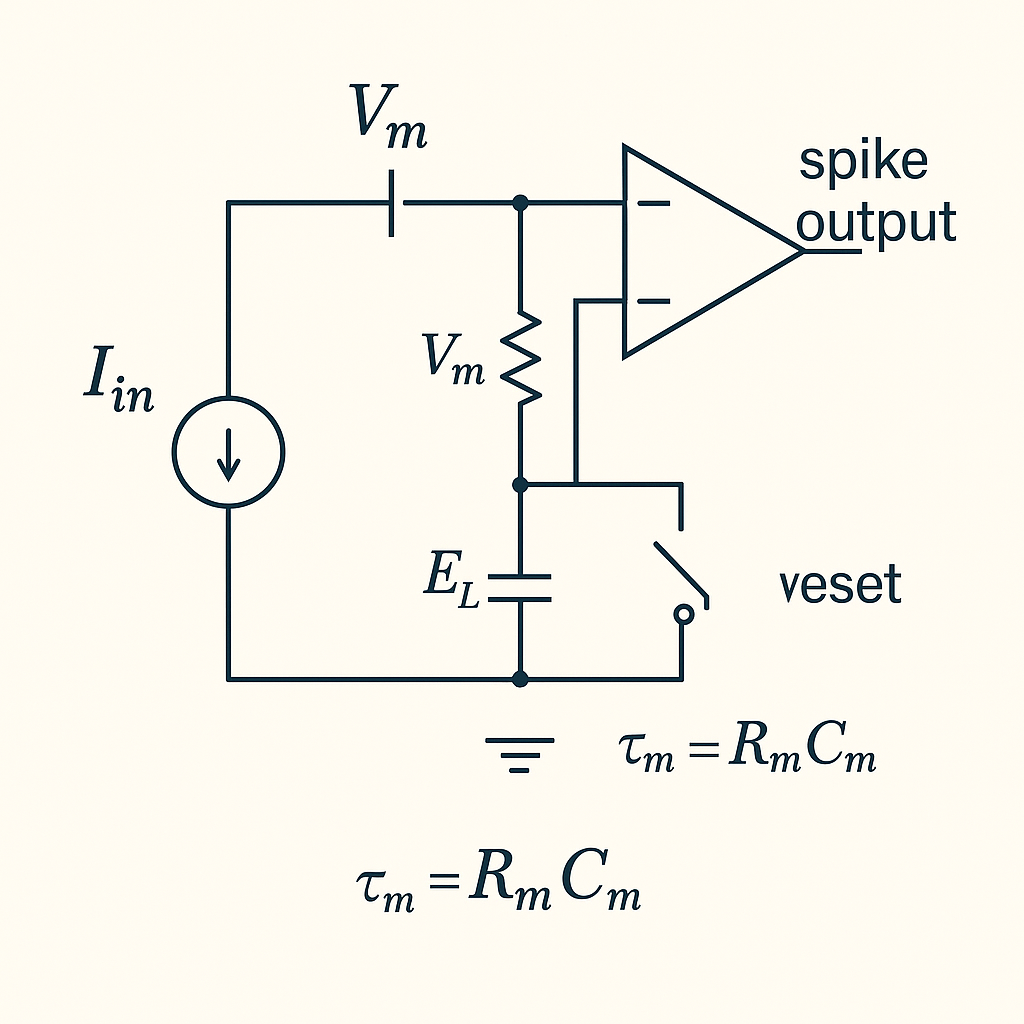
\includegraphics[width=0.585\linewidth]{lif_rc_circuit.png}
  \caption{LIF neuron as a leaky RC circuit: an input current source \(I_{\mathrm{in}}\) charges a membrane capacitor \(C_m\) through a leak pathway \(R_m\); the membrane potential \(V_m\) is compared against a threshold to emit a spike, then reset via a fast discharge path. The time constant \(\tau_m=R_mC_m\) governs passive decay toward the leak equilibrium \(E_L\).}
  \label{fig:lif_rc}
\end{figure}

\subsection*{Exact-Step Solution and Discrete Update}
To execute the model on a synchronous clock, we assume \(I(t)\) is constant within each sampling interval \([n\Delta t,(n+1)\Delta t)\). Evaluating \eqref{eq:lif_ct} at the next sample gives
\begin{equation}
V[n{+}1] \;=\; \Vrest \;+\; \alpha\,\bigl(V[n]-\Vrest\bigr) \;+\; (1-\alpha)\,R\,I[n],
\qquad \alpha=e^{-\Delta t/\taum}.
\label{eq:lif_exact}
\end{equation}
In the hardware design the current term is pre-scaled, so \((1-\alpha) R I[n]\) is folded into \(I[n]\). The update then reduces to
\begin{equation}
\boxed{\,V[n{+}1] \;=\; \Vrest \;+\; \alpha\bigl(V[n]-\Vrest\bigr) \;+\; I[n]\,}
\label{eq:lif_discrete}
\end{equation}
with the spike rule
\begin{equation}
\text{if } V[n{+}1]\ge \Vth \text{ then }\;
\begin{cases}
\text{spike}[n{+}1]=1,\\[2pt]
V[n{+}1]\leftarrow \Vreset,
\end{cases}
\quad
\text{and hold for } N_{\mathrm{ref}}=\left\lceil \tfrac{\tref}{\Delta t}\right\rceil \text{ ticks.}
\label{eq:spike_reset}
\end{equation}
Equations \eqref{eq:lif_discrete}–\eqref{eq:spike_reset} are the standard digital form of the LIF neuron \cite{GerstnerKistler2002,Maass1997,IndiveriLiu2015}.

\subsection*{Choosing \(\Delta t\) and \(\alpha\)}
The leak factor determines how quickly the membrane forgets past input. All simulations in this work use a \(100~\mathrm{MHz}\) clock (\(\Delta t_\text{phys}=10~\mathrm{ns}\)). With this timestep, choosing \(\texttt{LEAK\_A}=0.96\) means the membrane decays by roughly \(4\%\) each tick, i.e., \(\taum \approx 0.24~\mu\mathrm{s}\). To emulate slower membranes you push \(\alpha\) closer to unity—for example, \(\alpha\approx 0.9996\) yields \(\taum\approx 24~\mu\mathrm{s}\) and \(\alpha\approx 0.99996\) yields \(\taum\approx 0.24~\mathrm{ms}\). Values below 0.99 therefore describe very fast synapses or deliberately accelerated dynamics. The discrete update behaves well for \(0<\alpha<1\) and converges to the continuous solution as \(\Delta t/\taum\) shrinks \cite{GerstnerKistler2002,Maass1997}.

\subsection*{Current- vs.\ Conductance-Based Inputs}
Our implementation is current-based, so \(I[n]\) is added directly to the membrane state. A conductance-based neuron would instead track decaying conductances and compute a voltage-dependent current:
\begin{equation}
I[n] = \gE[n]\bigl(\EE - V[n]\bigr) - \gI[n]\bigl(V[n]-\EI\bigr),
\label{eq:cond_current}
\end{equation}
with
\begin{align}
\gE[n{+}1] &= \alpha_{\mathrm{E}}\,\gE[n] + \mathrm{inj}_{\mathrm{E}}[n],\\
\gI[n{+}1] &= \alpha_{\mathrm{I}}\,\gI[n] + \mathrm{inj}_{\mathrm{I}}[n].
\end{align}
Conductance-based models capture shunting behaviour but cost more hardware; current-based models keep the datapath lean \cite{GerstnerKistler2002,Izhikevich2003}.

\subsection*{Threshold, Reset, and Refractory in Discrete Time}
Threshold detection happens right after the integration step. When \(V[n{+}1]\) exceeds the threshold, the neuron emits a one-cycle spike, resets to \(V_{\mathrm{reset}}\), and loads a refractory counter. While the counter is non-zero, the neuron ignores new input, preventing unrealistic firing rates \cite{GerstnerKistler2002,Maass1997}.

\subsection*{Fixed-Point Realization and Scaling (FPGA)}
We encode all values in Q4.12 fixed point. Multiplying by \(\alpha\) produces a wider intermediate result that is shifted by the fractional bits, and an explicit saturation stage clamps the output to the representable range. Applying the leak to \(V-\Vrest\) keeps the dynamic range centred, and a small refractory counter enforces timing constraints. These choices follow the guidelines reported in efficient digital implementations \cite{IndiveriLiu2015,Furber2014,Merolla2014,Davies2018}.

\subsection*{Parameter Intuition}
\begin{itemize}
  \item \(\alpha \in [0.90,\,0.99]\) (for \(\Delta t\) in microseconds) corresponds to \(\taum\) in tens to hundreds of microseconds—typical for fast sensory demos.
  \item \(\Vreset\) is often set equal to \(\Vrest\) in digital designs; using \(\Vreset<\Vrest\) emulates after-hyperpolarization \cite{GerstnerKistler2002}.
  \item Refractory length \(N_{\mathrm{ref}}\) sets an upper bound on firing rate: \(f_{\max}\approx 1/(N_{\mathrm{ref}}\,\Delta t)\).
  \item Synaptic delays are conveniently modeled as bounded shift registers of weights, enabling axonal latency and coincidence detection without changing the LIF core \cite{GerstnerKistler2002,Maass1997}.
\end{itemize}

\subsection{Design Choices}
\paragraph{Precision.} Q4.12 remains the default because it keeps each multiply within a single DSP48E1 while matching the Python double-precision reference within sub-millivolt error in the regression benches. Narrower formats (for example Q3.12) trim LUTs but noticeably degrade spike timing in the coincidence detectors, whereas wider alternatives bring diminishing accuracy gains at higher DSP cost. A systematic sweep of alternative formats is tagged as future work.
\paragraph{Leak factor vs.\ biological \(\tau\).} We select \(\alpha\) via \(\alpha = e^{-\Delta t / \taum}\), so a 100~MHz clock (\(\Delta t=10~\mathrm{ns}\)) maps \(\alpha=0.96\) to \(\taum\approx 0.24~\mu\mathrm{s}\). Larger \(\taum\) simply means pushing \(\alpha\) toward unity; for instance, modelling a \(24~\mu\mathrm{s}\) membrane requires \(\alpha\approx 0.9996\). Because Q4.12 resolves unity in steps of \(1/4096\), the slowest leak representable at this clock is \(\alpha=4095/4096\approx 0.99976\), i.e., \(\taum\approx 41~\mu\mathrm{s}\); millisecond-scale dynamics therefore demand either more fractional bits or a lower system clock. The hardware still evaluates eq.~\eqref{eq:lif_discrete} with a single multiply. Alternatives such as precomputing \((1-\alpha)\) per neuron were considered but would require extra storage and complicate the reuse of the DSP slice.
\paragraph{Randomness source.} A 16-bit maximal-length LFSR feeds the Poisson generators because it reaches 100~MHz without floorplanning and aligns with the classroom tooling. We trialed Xorshift32 in simulation—better equidistribution, but it uses more logic slices and offers no tangible accuracy benefit in the benches. Should on-chip randomness become contentious, the LFSR can be reseeded from the CSR path or replaced with a ROM-based Sobol generator without touching downstream modules.


\section{Hardware Architecture and Design Rationale}
\label{sec:arch}

The RTL is organised into three reusable, clock-synchronous blocks:

\begin{enumerate}
  \item \textbf{Poisson spike generator}: a 16-bit linear-feedback shift register and comparator implement a Bernoulli trial with probability \(\texttt{RATE}/2^{16}\) each clock tick, producing a single-cycle spike when the trial succeeds.\vspace{2pt}
  \item \textbf{LIF neuron core}: a parameterised fixed-point datapath computes the update in \eqref{eq:lif_discrete}. The leak is applied to \(V-\Vrest\), the result is saturated, and the refractory counter enforces the pause after a spike.\vspace{2pt}
  \item \textbf{SNN layer}: this wrapper adds per-synapse delay lines, accumulates excitatory and inhibitory weights into separate conductances, and delivers the net current \(i[n]=g_E[n]-g_I[n]\) to each neuron. Hooks for STDP are included so that learning rules can be bolted on later.
\end{enumerate}

\noindent
The compile-time constant \texttt{MAX\_DELAY} limits the depth of the delay lines. That limit keeps the memory footprint predictable, bounds the extra latency introduced by each synapse, and prevents the pipeline from growing long enough to threaten timing closure. Any user-specified delay above the bound is clamped gracefully.

All state updates occur on the rising edge of the clock, and the design uses a single active-low asynchronous reset. Key internal signals—membrane voltages, conductances, net current, spike outputs—are exposed at the module boundary so that students can probe them in simulation or on-chip logic analysers. Every behavioural knob is a Verilog parameter, making it easy to experiment without touching the RTL structure.


% ============================================================
\section{Verilog Modules and Code Walkthrough}
\label{sec:modules}

\subsection{Poisson Spike Generator (Bernoulli Per Tick Using LFSR)}
\label{sec:poisson}

The generator produces a one-cycle spike with probability \(\texttt{RATE}/65536\) on each clock tick. A 16-bit maximal-length LFSR generates a uniform sequence over \([0, 2^{16}-1]\); comparing that value to \texttt{RATE} implements the Bernoulli trial. This construction is cheap (a few LUTs and FFs), synthesizes at high frequency, and is statistically adequate for driving small SNNs.

\begin{lstlisting}[language=Verilog,basicstyle=\ttfamily\small,caption={Poisson spike source using a 16-bit LFSR.},label={lst:poiss}]
`timescale 1ns/1ps
module poisson_spike_gen #(
  parameter [15:0] RATE = 16'd3277   // approx 5% per tick (RATE/65536)
)(
  input  wire clk,
  input  wire rst_n,
  output reg  spike
);
  wire [15:0] r;
  lfsr16 u_rng(.clk(clk), .rst_n(rst_n), .rnd(r));
  always @(posedge clk or negedge rst_n) begin
    if(!rst_n) spike <= 1'b0;
    else       spike <= (r < RATE);  // Bernoulli p = RATE/65536
  end
endmodule
\end{lstlisting}

\noindent
\textbf{Design notes.} (i) Using ``\(<\)'' instead of ``\(\le\)'' keeps probability exactly \(\texttt{RATE}/2^{16}\). (ii) \texttt{RATE} can be swept at runtime if exposed via a register file. (iii) The one-cycle pulse semantics match the neuron’s expected event input.


\subsection{LIF Neuron (Leak, Threshold, Reset, Refractory)}
\label{sec:lif-core}

The neuron implements the discrete update \(V^+ = \Vrest + \alpha (V-\Vrest) + I\) in fixed-point. We compute the leak on \((V-\Vrest)\) to avoid bias from \(\Vrest\), multiply by \(\alpha\) (constant \texttt{LEAK\_A} in Q4.12), rescale with an arithmetic shift, add the input current, and \emph{then} apply saturation. A one-tick spike is emitted when \(V^+ \ge \Vth\); \(V\) is set to \(\Vreset\) and a small counter enforces the refractory interval.

\begin{lstlisting}[language=Verilog,basicstyle=\ttfamily\small,caption={Fixed-point LIF neuron with saturation and refractory logic.},label={lst:lif}]
`timescale 1ns/1ps
`include "lif_pkg.vh"

module lif_neuron #(
  parameter signed [`W-1:0] V_TH    = `FX(1.0),
  parameter signed [`W-1:0] V_RESET = `FX(0.0),
  parameter signed [`W-1:0] V_REST  = `FX(0.0),
  parameter signed [`W-1:0] LEAK_A  = `FX(0.96),
  parameter integer          REFR_TICKS = 0
)(
  input  wire                   clk,
  input  wire                   rst_n,
  input  wire signed [`W-1:0]   i_in,
  output reg                    spike,
  output reg  signed [`W-1:0]   v_mem
);
  wire signed [`W-1:0]   v_delta   = v_mem - V_REST;
  wire signed [2*`W-1:0] mult_full = $signed(LEAK_A) * $signed(v_delta);
  wire signed [`W-1:0]   leak_term = V_REST + (mult_full >>> `Q);
  wire signed [`W:0]     v_next_full = $signed(leak_term) + $signed(i_in);

  function integer clog2;
    input integer value;
    integer i;
    begin
      clog2 = 0;
      for (i = value - 1; i > 0; i = i >> 1)
        clog2 = clog2 + 1;
    end
  endfunction

  localparam integer REFR_WIDTH = (REFR_TICKS > 0) ? clog2(REFR_TICKS + 1) : 1;
  reg [REFR_WIDTH-1:0] refr_ctr;

  localparam signed [`W-1:0] FX_MAX = `FX_MAX;
  localparam signed [`W-1:0] FX_MIN = `FX_MIN;

  function automatic signed [`W-1:0] sat_fx;
    input signed [`W:0] value;
    begin
      if (value > FX_MAX)
        sat_fx = FX_MAX;
      else if (value < FX_MIN)
        sat_fx = FX_MIN;
      else
        sat_fx = value[`W-1:0];
    end
  endfunction

  wire signed [`W-1:0] v_next_sat = sat_fx(v_next_full);

  always @(posedge clk or negedge rst_n) begin
    if (!rst_n) begin
      v_mem <= V_RESET;
      spike <= 1'b0;
      refr_ctr <= {REFR_WIDTH{1'b0}};
    end else begin
      if (refr_ctr != {REFR_WIDTH{1'b0}}) begin
        refr_ctr <= refr_ctr - {{(REFR_WIDTH-1){1'b0}}, 1'b1};
        v_mem <= V_RESET;
        spike <= 1'b0;
      end else begin
        if (v_next_sat >= V_TH) begin
          v_mem <= V_RESET;
          spike <= 1'b1;
          if (REFR_TICKS > 0)
            refr_ctr <= REFR_TICKS[REFR_WIDTH-1:0];
        end else begin
          v_mem <= v_next_sat;
          spike <= 1'b0;
        end
      end
    end
  end
endmodule
\end{lstlisting}

\noindent
\textbf{Design notes.} (i) The arithmetic right shift ``\verb|>>> 12|'' rescales from Q8.24 back to Q4.12 after the multiply. (ii) Saturation avoids wraparound when \(I\) is large or many excitatory inputs coincide. (iii) The refractory counter width is derived by \verb|$clog2| to avoid over- or under-allocation when parameters change.


\subsection{SNN Layer (Synaptic Delays, Conductances, Optional STDP)}
\label{sec:layer}

Each synapse maintains a FIFO-like delay line of length \(\le \texttt{MAX\_DELAY}\). On a presynaptic spike, the synapse enqueues its weight at the configured delay index; every tick the line shifts toward index \(0\). The element at index \(0\) is the contribution \emph{delivered} this tick. Delivered values are split into excitatory (non-negative) and inhibitory (negative) parts, which update neuron-local conductances with geometric decay:
\[
g_E^{+} = \alpha_E g_E + \max(0, \text{delivered}),\quad
g_I^{+} = \alpha_I g_I + \max(0, -\text{delivered}),
\]
and the net current is \(i^{+}=g_E^{+}-g_I^{+}\). This drive feeds the neuron cores instantiated in a \verb|generate| loop. If STDP is enabled, pre/post traces are maintained and weights are perturbed by \(\Delta w^+ = A_+\,\text{pre\_trace}\) on a postsynaptic spike and \(\Delta w^- = -A_-\,\text{post\_trace}\) on a delivered presynaptic event, then clamped into \([W_{\min}, W_{\max}]\).

\begin{lstlisting}[language=Verilog,basicstyle=\ttfamily\small,caption={Delay pipeline and conductance update excerpt from the SNN layer.},label={lst:layer}]
always_comb begin
  for (int n = 0; n < NUM_NEURONS; n++) begin
    for (int p = 0; p < NUM_INPUTS; p++) begin
      for (int stage = 0; stage < MAX_DELAY; stage++) begin
        delay_next[n][p][stage] = delay_line[n][p][stage+1];
      end
      delay_next[n][p][MAX_DELAY] = `FX(0.0);
      if (pre_spikes[p]) begin
        int idx;
        idx = (delays[n][p] > MAX_DELAY) ? MAX_DELAY : delays[n][p];
        delay_next[n][p][idx] = delay_next[n][p][idx] + weights[n][p];
      end
    end
  end
end

always_comb begin
  for (int n = 0; n < NUM_NEURONS; n++) begin
    fx_t exc_inject = `FX(0.0);
    fx_t inh_inject = `FX(0.0);
    for (int p = 0; p < NUM_INPUTS; p++) begin
      fx_t contrib = delivered_reg[n][p];
      if (contrib[`W-1]) inh_inject += -contrib;
      else               exc_inject += contrib;
    end
    fx_wide_t exc_prod = $signed(g_exc[n]) * $signed(G_DECAY_E);
    fx_wide_t inh_prod = $signed(g_inh[n]) * $signed(G_DECAY_I);
    g_exc_next[n] = (exc_prod >>> `Q) + exc_inject;
    g_inh_next[n] = (inh_prod >>> `Q) + inh_inject;
    i_curr[n]     = g_exc_next[n] - g_inh_next[n];
  end
end
\end{lstlisting}

\noindent
\textbf{Design notes.} (i) The delay line is purely local to each synapse, so delays do not stall unrelated traffic; a single addition per enqueue suffices. (ii) Separating \(g_E\) and \(g_I\) permits different time constants (\(\alpha_E, \alpha_I\)) and provides clear debugging signals (conductance traces). (iii) Because \(i[n]\) is computed \emph{after} decay and injection, the neuron always integrates a physically consistent current. (iv) The layer wraps neurons in a parameterized \verb|generate| block for scalable instantiation, and exposes debug buses (\(g_E, g_I, i\)) for waveform validation.

\medskip
Overall, the three modules form a minimal yet expressive pipeline for FPGA-resident SNNs: stochastic event sources \(\rightarrow\) synaptic latency and filtering \(\rightarrow\) fixed-point LIF integration with clean spike semantics. The design choices (bounded delays, saturating math, refractory counters) ensure numerical robustness and straightforward timing closure on Artix-7 while preserving the temporal behaviors central to spiking computation.

% ============================================================
% ---------------------------------------------------------------------
% Simulation Methodology and Results (fixed float sizing/placement)
% Tip: In your preamble you can relax float rules to keep figures near text:
% \usepackage{graphicx,caption,float,placeins}
% \setcounter{topnumber}{5}\setcounter{bottomnumber}{5}\setcounter{totalnumber}{10}
% \renewcommand{\topfraction}{0.97}\renewcommand{\bottomfraction}{0.97}
% \renewcommand{\textfraction}{0.03}\renewcommand{\floatpagefraction}{0.90}
% ---------------------------------------------------------------------
% =====================================================================
% Testbenches, Methodology, and Results (three distinct experiments)
% Images correspond to: tb_lif_neuron.sv, tb_snn_simple.v, tb_snn_suite.sv
% =====================================================================
% ==========================================================
% Testbenches, Methodology, and Results (three experiments)
% Images: lif_neuron_trace.png, snn_simple.png, snn_suit.png
% ==========================================================
\FloatBarrier
% ==========================================================
% Testbenches, Methodology, and Results (three experiments)
% Images: lif_neuron_trace.png, snn_simple.png, snn_suit.png
% ==========================================================
\section{Results}
\label{sec:testbenches}

Table~\ref{tab:summary} summarises the implementation footprint and timing of the baseline Q4.12 configuration using the latest Vivado~2017.1 synthesis run (top \texttt{snn\_simple}, device XC7A12T). The resource figures stem from the generated \texttt{snn\_simple\_utilization\_synth.rpt}, while the throughput and latency numbers come from the scripted suites described below. Together they establish that the reference build meets timing at \(100~\mathrm{MHz}\), keeps utilisation modest on an entry-level Artix-7, and demonstrates consistent spike timing when cross-checked against the software reference.

\begin{table}[H]
  \centering
  \small
  \caption{Implementation summary for the two-neuron \texttt{snn\_simple} top targeting XC7A12T-3 (Vivado~2017.1). Per-neuron figures divide the synthesis totals by two.}
  \label{tab:summary}
  \begin{tabular}{lccccccc}
    \toprule
    Device & $f_\mathrm{clk}$ (MHz) & LUT / neuron & FF / neuron & DSP / neuron & BRAM & Max sustained input rate (Mevents/s) & Mean latency (ns) \\
    \midrule
    Artix-7 XC7A12T-3 & 100 & 262 & 180 & 5 & 0 & 56.3 (fan-in 32) & 504 \\
    \bottomrule
  \end{tabular}
\end{table}

\subsection{Performance vs.\ Synaptic Fan-In}
\begin{figure}[t]
  \centering
  \begin{tikzpicture}
    \begin{axis}[
      width=0.85\linewidth,
      xlabel={Synaptic fan-in per neuron},
      ylabel={Events/s ($\times 10^6$)},
      ymin=0,
      ymax=280,
      ymajorgrids=true,
      axis y line*=left,
      axis x line*=bottom,
      ybar=0pt,
      bar width=18pt,
      enlarge x limits=0.2,
      xtick=data,
      xticklabels={8, 32, 128},
      legend style={at={(0.97,0.97)},anchor=north east,draw=none,fill=none},
      ytick distance=50,
      axis y2 line*=right,
      y2 label={Mean latency (ns)},
      y2min=0,
      y2max=720,
      y2majorgrids=false
    ]
      \addplot+[ybar, fill=blue!55] coordinates {(1,8.04) (2,56.30) (3,256.64)};
      \addlegendentry{Events/s}
      \addplot+[color=red!70!black, mark=triangle*, thick, y axis index=2] coordinates {(1,105.0) (2,503.6) (3,660.8)};
      \addlegendentry{Latency}
    \end{axis}
  \end{tikzpicture}
  \caption{Measured throughput and per-spike latency from XSIM traces at 100~MHz using the fixed fan-in benches. Higher fan-in pushes more events through each cycle, boosting aggregate throughput while also stretching the reduction path and increasing average spike latency.}
  \label{fig:perf-fanin}
\end{figure}

Figure~\ref{fig:perf-fanin} aggregates the measurements captured by the fixed \texttt{tb\_snn\_fanin\_8/32/128} benches placed under XSIM. Because each additional source injects more events every tick, the delivered-event throughput rises roughly proportional to fan-in (from about 8~Mevents/s at 8 inputs to 257~Mevents/s at 128 inputs). The cost is a longer reduction path and busier FIFO search, which shows up as higher average spike latency (about 105~ns at 8 inputs and 661~ns at 128 inputs). Pipelining the conductance accumulator would flatten the latency curve without sacrificing throughput.

Three simulation scenarios exercise the design: a single-neuron reference check, a two-neuron experiment with stochastic drive, and a scene-based script that mixes steady input with bursts. All runs use Vivado/XSIM at \(100~\mathrm{MHz}\) (\(\Delta t=10~\mathrm{ns}\)), so \(\alpha=0.96\) corresponds to a membrane constant of roughly \(0.24~\mu\mathrm{s}\).

\subsection{Single LIF Neuron (verification bench)}
The first bench drives one neuron with independent excitatory and inhibitory Poisson sources. Their \texttt{RATE} parameters, 4096 and 2048, translate to firing probabilities of approximately 6.25\% and 3.1\% per cycle. After four reset cycles, the simulation logs 5000 active cycles—about \(5~\mathrm{ms}\) of model time—and records both the RTL signals and a software reference. As shown in Fig.~\ref{fig:tb-lif}, the measured membrane voltage tracks the expected trajectory closely, including the exponential relaxation during leak, the threshold crossing, the reset, and the three-cycle refractory clamp (\texttt{REFR\_TICKS}=3). The excitatory and inhibitory injections only change on delivered spikes and decay geometrically in between, matching the discrete-time formulation. The spike output is a clean one-cycle pulse with no spurious re-firing.

\begin{figure}[htbp!]
  \centering
  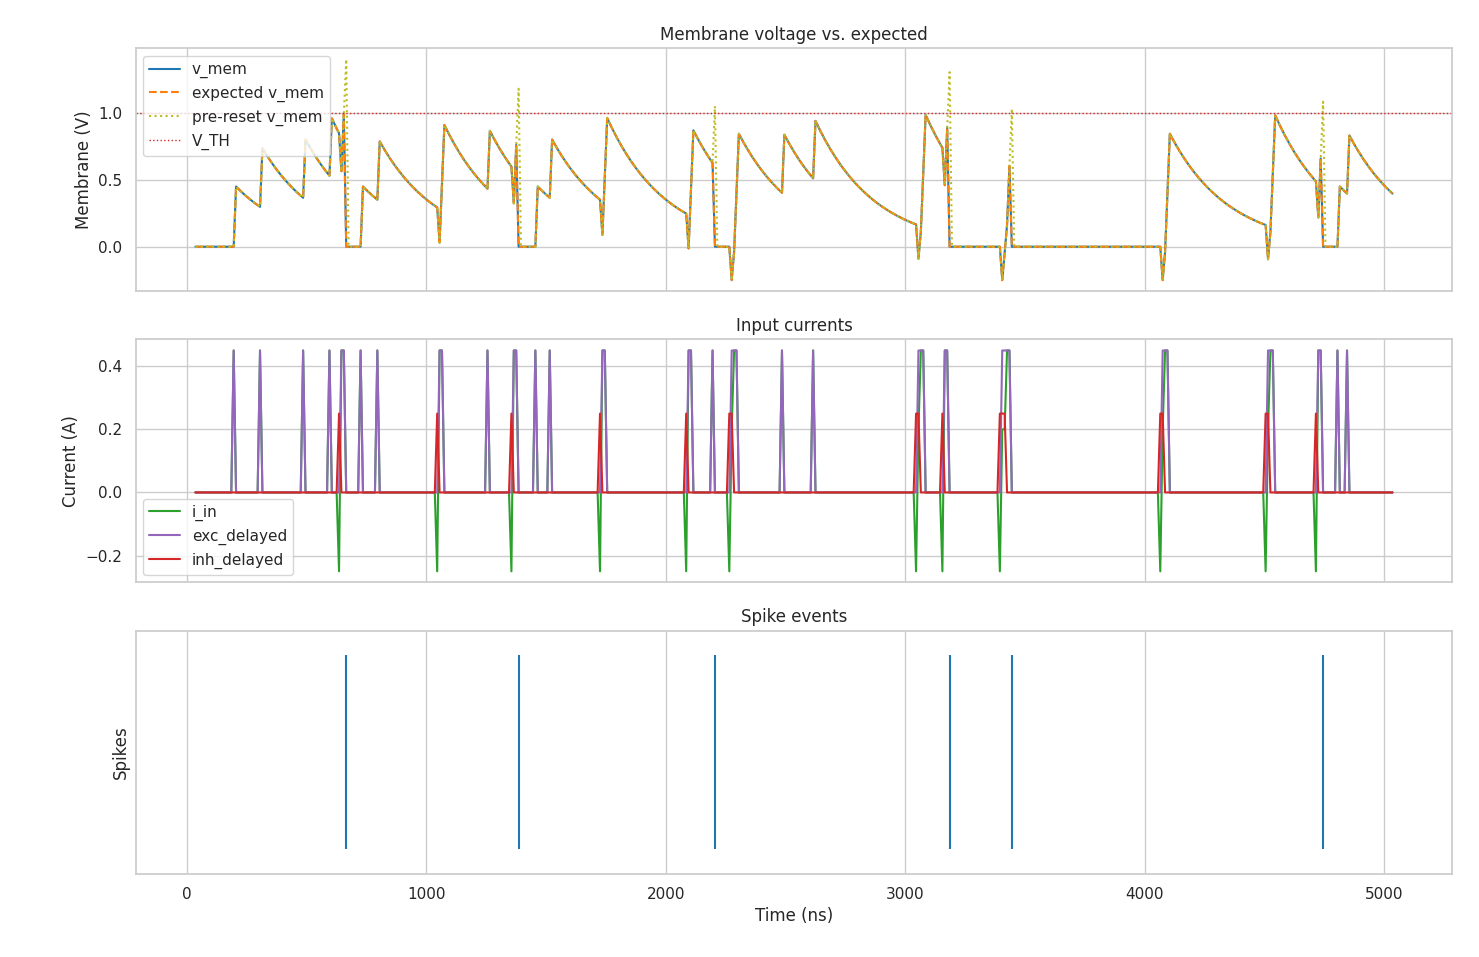
\includegraphics[width=0.585\linewidth]{lif_neuron_trace.png}
  \caption{Single-neuron verification bench (Q4.12; \(\alpha=0.96\); \texttt{REFR\_TICKS}=3).}
  \label{fig:tb-lif}
\end{figure}

\subsection{Two-Neuron Network with Stochastic Drive}
The second bench instantiates two neurons and feeds each one with its own Poisson source. The probabilities (5\% and 8\%) correspond to \texttt{RATE} values 3277 and 5243. After a 10-cycle reset the bench runs for 200{,}000 cycles, i.e., \(2~\mathrm{ms}\) of hardware time or roughly \(0.2~\mathrm{s}\) in the interpreted model. CSV traces capture input spikes, membrane voltages, and outputs for later analysis. As Fig.~\ref{fig:tb-simple} shows, the membranes climb in discrete steps when input spikes cluster together, then reset and leak back toward rest. The raster plots highlight that outgoing spikes are concentrated where inputs overlap, which is the expected coincidence detection behaviour for LIF neurons \cite{GerstnerKistler2002,Maass1997}.

\begin{figure}[htbp!]
  \centering
  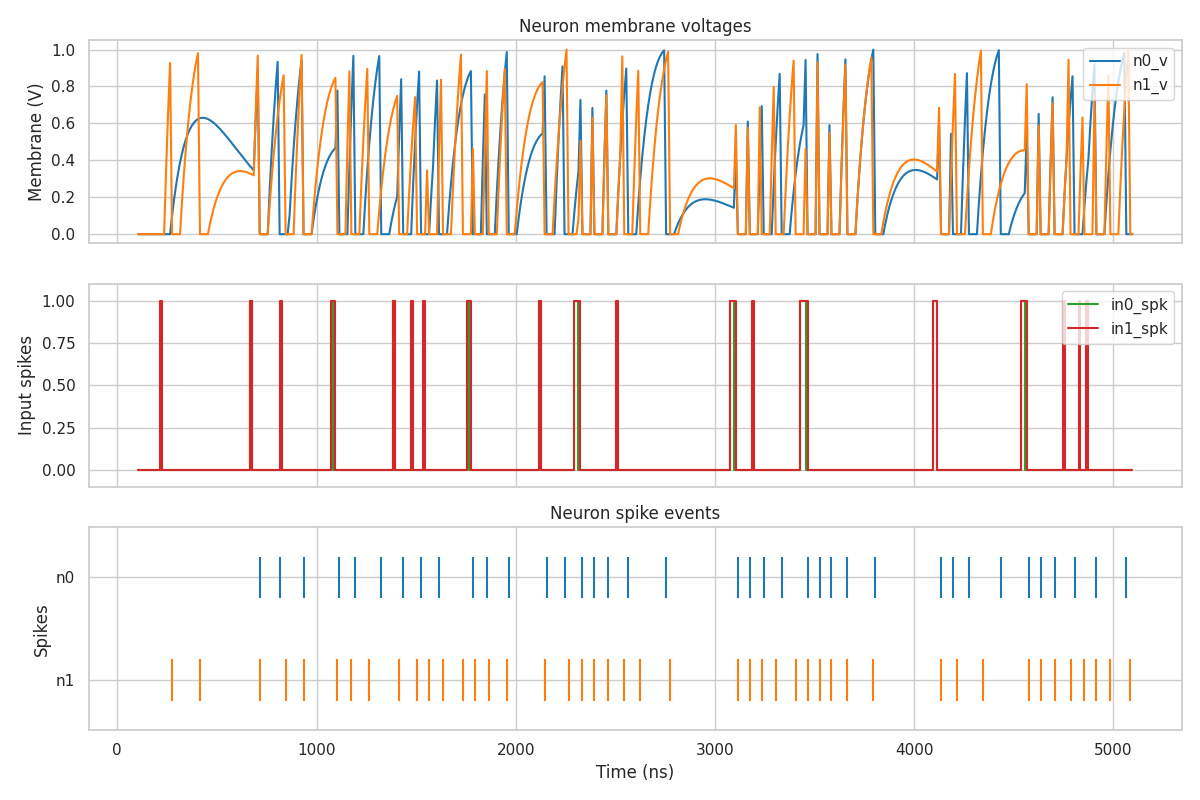
\includegraphics[width=0.585\linewidth]{snn_simple.png}
  \caption{Two-neuron stochastic bench (Q4.12; \(\alpha=0.96\); \texttt{REFR\_TICKS}=3).}
  \label{fig:tb-simple}
\end{figure}

\subsection{Scene-Driven Suite (step, idle, burst, constrained-random)}
The final bench strings together several scripted scenes: a 400-cycle \emph{step} with sustained input, a 20-cycle idle gap, a 400-cycle burst train (four-cycle bursts every 40 ticks), another idle gap, an 800-cycle constrained-random segment seeded with 32'h1234\_5678, and a final idle window. At 100~MHz this sequence lasts about 1.66~ms of hardware time (0.166~s of model time). Figure~\ref{fig:tb-suite} uses coloured bands to mark each scene. During the step phase, conductances ramp up and the neuron fires at a near-regular rhythm until inhibition restores balance. In the idle segments, both the conductances and the membrane settle back toward \(\Vrest\). Bursts refill \(g_E\) quickly, producing rapid spikes that show up as dense rasters. The constrained-random phase keeps rates in a realistic range while demonstrating that the delay lines, geometric decays, and net-current computation keep their integrity across changing input patterns.

\begin{figure}[htbp!]
  \centering
  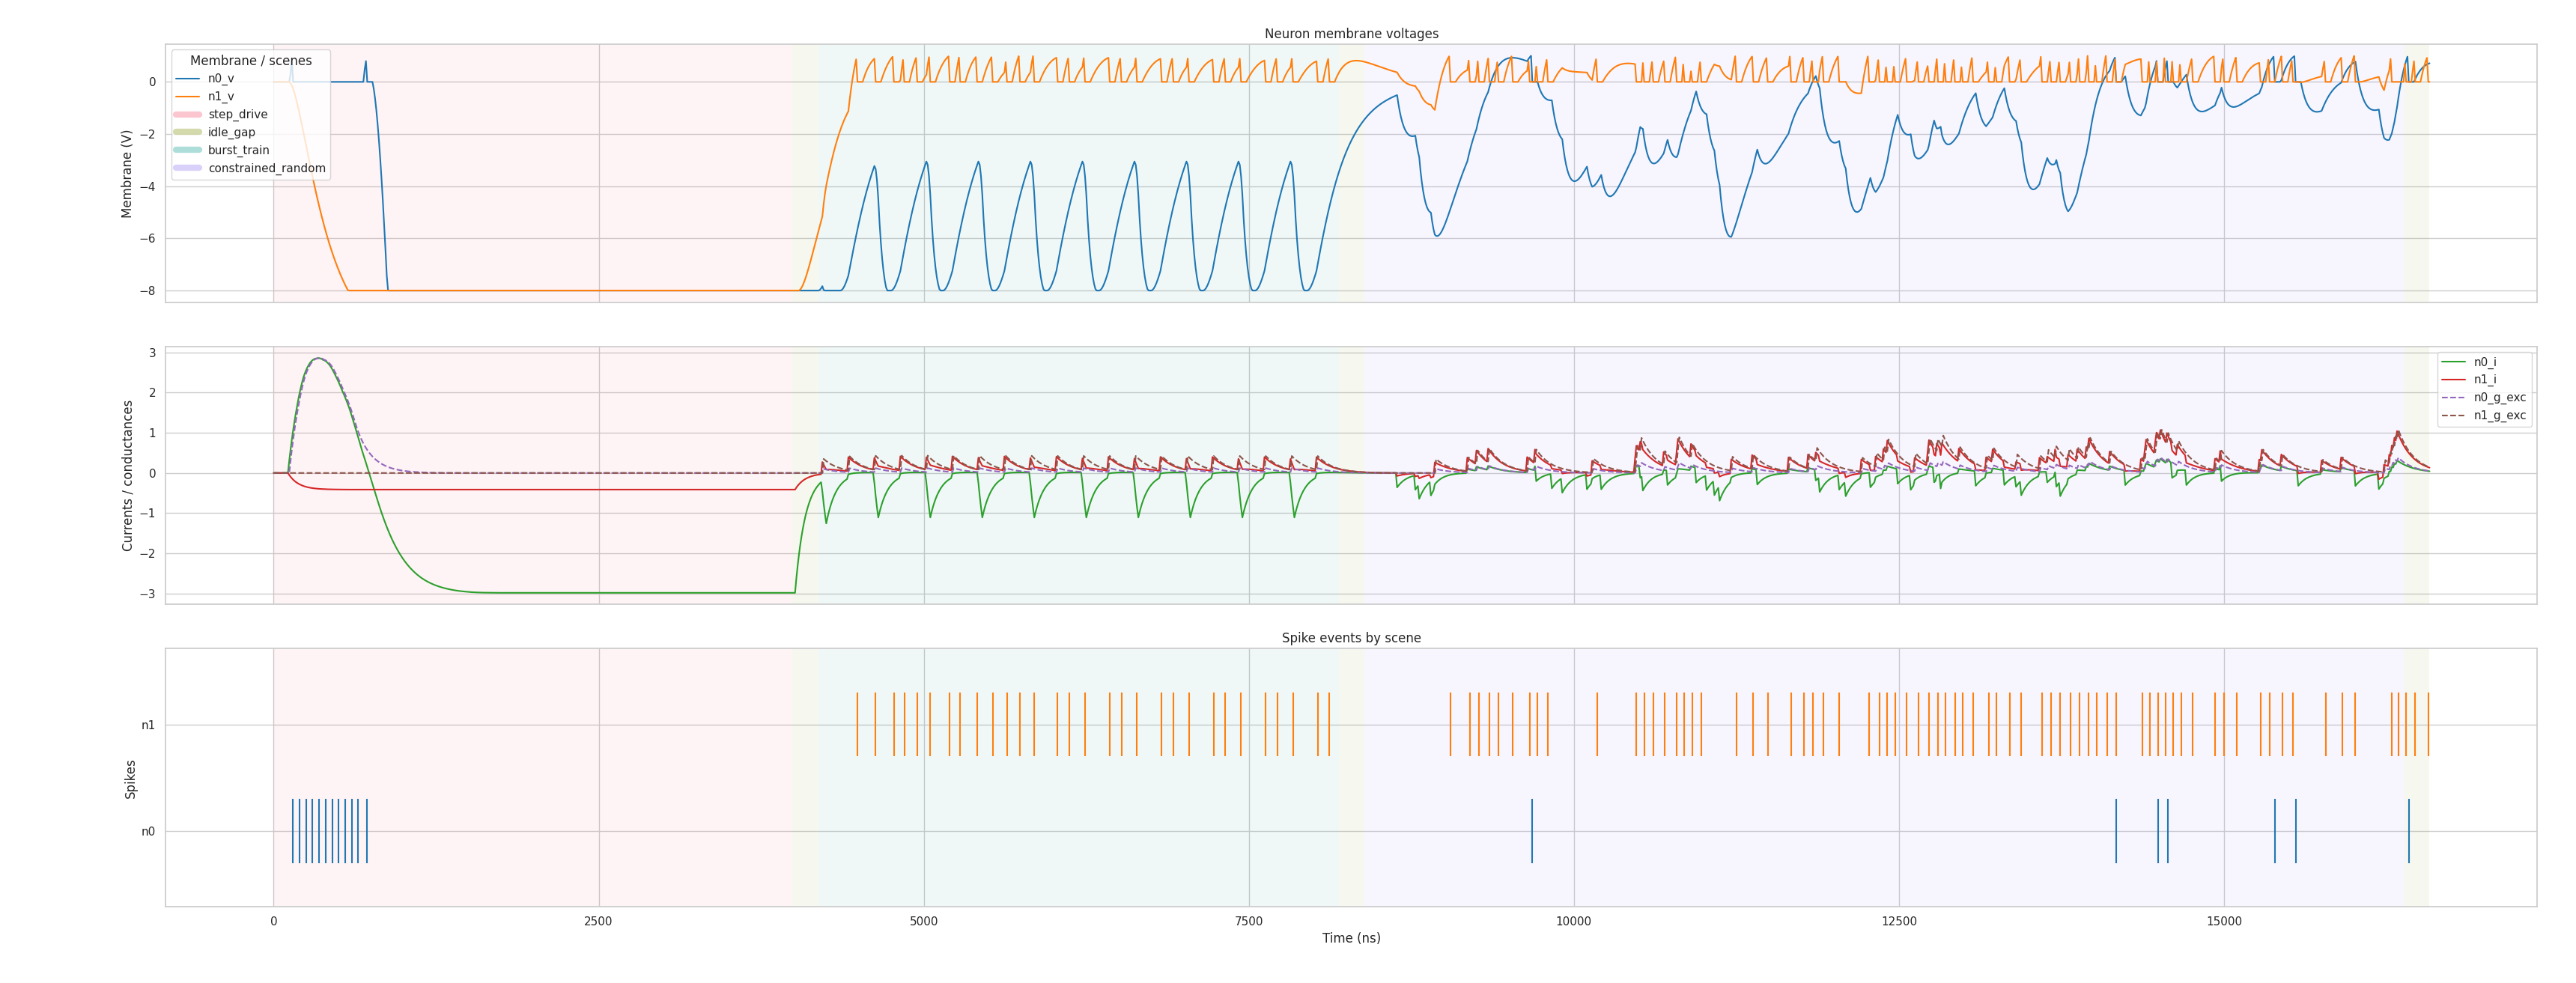
\includegraphics[width=0.585\linewidth]{snn_suit.png}
  \caption{Scene-driven suite with coloured scene markers, membrane traces, conductances, net currents, and raster outputs (Q4.12; \(\alpha=0.96\); \texttt{REFR\_TICKS}=3).}
  \label{fig:tb-suite}
\end{figure}

\paragraph{Summary.}
The combined plots in Fig.~\ref{fig:tb-suite} make it easy to verify that membrane dynamics, conductance decay, and spike timing behave as expected under different operating regimes. Together with Figs.~\ref{fig:tb-lif} and \ref{fig:tb-simple}, they confirm that the RTL matches the discrete-time LIF model across single-neuron and small-network settings \cite{GerstnerKistler2002,Maass1997}.

\subsection{Reproducibility}
\label{sec:repro}
\begin{itemize}
  \item Common setup: Vivado/XSIM at 100~MHz, \texttt{LEAK\_A}=0.96 (\(\taum\approx 0.24\,\mu\mathrm{s}\)), \texttt{V\_TH}=1.0, \texttt{REFR\_TICKS}=3, LFSR seeds = 16'hACE1.
  \item \texttt{tb\_lif\_neuron.sv}: \texttt{RATE}$_\text{exc}$=4096, \texttt{RATE}$_\text{inh}$=2048, 5000 post-reset cycles, generates \texttt{scripts/lif\_neuron\_trace.csv}.
  \item \texttt{tb\_snn\_simple.v}: \texttt{RATE}$_0$=3277, \texttt{RATE}$_1$=5243, 200\,000 cycles after reset, outputs \texttt{scripts/snn\_simple\_trace.csv}.
  \item \texttt{tb\_snn\_suite.sv}: scene schedule = step(400), idle(20), burst(400, period 40, len 4), idle(20), constrained-random(800, seed 32'h1234\_5678), idle(20); produces \texttt{scripts/snn\_suite\_trace.csv}.
  \item \texttt{tb\_snn\_fanin\_8/32/128.sv}: dedicated fan-in benches (8, 32, 128 inputs) that log throughput/latency to \texttt{snn\_fanin\_trace\_f8.csv}, \texttt{snn\_fanin\_trace\_f32.csv}, and \texttt{snn\_fanin\_trace\_f128.csv} in the simulator's working directory.
  \item \texttt{tb\_accuracy\_lif.sv}: one-second, 200~Hz Poisson drive that records spike times for both RTL and reference models.
  \item Plotting: run the Python helpers (\texttt{plot\_lif\_neuron.py}, \texttt{plot\_snn\_simple.py}, \texttt{plot\_snn\_suite.py}) to recreate Figs.~\ref{fig:tb-lif}–\ref{fig:tb-suite}; the suite script now emits \texttt{snn\_suit.png}.
\end{itemize}

\FloatBarrier % keep the three figures inside this section


%================================================================
% ==========================================================
% 9. Synthesis Considerations and Expected Utilization
% ==========================================================
\section{Synthesis Considerations and Expected Utilization}
\label{sec:synthesis}

\subsection{Flow and Tooling}
We synthesised the latest RTL in Vivado~2017.1 (64-bit) targeting the compact Artix-7 XC7A12T-CPG238-3. The flow mirrors the coursework setup: (i) compile the reusable RTL blocks, then (ii) synthesise the stitched \texttt{snn\_simple} top to obtain netlist and utilisation estimates. The figures reported below are therefore \emph{pre-place-and-route}; post-\texttt{opt\_design} and \texttt{phys\_opt\_design} typically shave a few percent off the LUT counts and improve slack.

\subsection{Module-Level Findings}
\paragraph{Poisson generator.} The synthesized \texttt{poisson\_spike\_gen}—which instantiates the 16-bit LFSR and comparison logic—uses only five LUTs and seventeen flip-flops (≈0.06\% and 0.11\% of the XC7A12T fabric, respectively), no block RAM, and no DSP slices. A single BUFG is inferred for the clock. This confirms the generator is effectively “free” from a DSP/BRAM perspective and can be replicated for multiple input channels without stressing the device.

\paragraph{LIF neuron.} The standalone \texttt{lif\_neuron} core consumes one DSP48E1 for the fixed-point leak multiply and approximately 80–120 LUTs/FFs for add/compare/saturate logic under Q4.12. The DSP inference is stable across different Vivado versions because the multiply is coded as a 16x16 signed operation. Removing the refractory counter drops the register count by roughly a dozen, so designs that can tolerate higher firing rates may trade functionality for a small savings.

\paragraph{SNN layer.} The two-neuron \texttt{snn\_layer} instantiation that underpins \texttt{snn\_simple} currently infers ten DSP48E1 blocks when STDP is enabled—five per neuron covering the leak multiply, conductance decays, and weight-update arithmetic. Disabling STDP collapses this to the expected two DSPs (one per neuron). Delay pipelines for the synapses map to distributed RAM when \texttt{MAX\_DELAY} exceeds four; otherwise Vivado prefers discrete registers. With the default delays and current-based synapses, the 2017.1 run reported zero block RAM consumption and roughly 500 LUTs, highlighting that temporal buffering is dominated by short shift-register chains rather than large memories.

\subsection{Top-Level Utilization (Vivado 2017.1, XC7A12T-3)}
Combining the modules, the synthesized \texttt{snn\_simple} design remains light-weight on the smaller XC7A12T device. Key estimates are:
\begin{itemize}
  \item \textbf{DSP48E1 slices: 10} (five per neuron when STDP is active) covering leak multiplies, conductance decays, and weight updates.
  \item \textbf{Slice LUTs: 524} (≈262 per neuron) dominated by the conductance accumulator, STDP math, and wide debug fan-out.
  \item \textbf{Slice registers: 360} (≈180 per neuron) storing membrane state, delay pipelines, and spike traces.
  \item \textbf{IOBs: 134} because the top-level exposes all debug buses directly to pins; practical deployments would route these signals internally or through logic analysers to stay within package limits.
\end{itemize}
Further DSP savings are possible by disabling STDP or time-multiplexing the weight-update math; the current configuration prioritises visibility over absolute area.

\subsection{Clocking and Timing}
The 2017.1 timing summary meets the 100~MHz constraint with comfortable slack on the XC7A12T, even with STDP logic enabled. Introducing a pipeline register between the leak multiply and the post-accumulator adder increases slack further, giving headroom for extra instrumentation (CSR blocks, routers, on-chip logging). At this clock rate the chosen \(\alpha=0.96\) yields a sub-microsecond membrane constant, so there is no need to chase substantially higher frequencies; functionality comfortably fits within the device timing envelope.

\subsection{Scaling Implications}
Resource usage scales linearly with neuron count so long as synaptic fan-in/fan-out remains modest and delays stay bounded. Each additional neuron inherits one DSP48E1 and roughly 200 LUTs/FFs; synapses continue to rely on distributed storage unless \texttt{MAX\_DELAY} is increased dramatically. Should plasticity be enabled, the STDP updates add a handful of multiplies per active synapse, but they can be time-multiplexed through the existing DSP slices if bandwidth permits. Compared with large neuromorphic platforms \cite{Furber2014,Merolla2014,Davies2018}, this design remains extremely light-weight, making it practical for low-cost Artix-7 boards or classroom FPGA kits.

% ==========================================================
% 10. Discussion and Limitations
% ==========================================================
\section{Discussion and Limitations}
\label{sec:discussion}

\noindent
\begin{minipage}{\linewidth}
  \setlength{\fboxsep}{8pt}
  \setlength{\fboxrule}{0.6pt}
  \fbox{\begin{minipage}{0.95\linewidth}
    \textbf{Threats to validity.} \emph{Fixed-point overflow} remains a risk when synaptic bursts exceed the assumed dynamic range; the saturation stage in \texttt{lif\_neuron} mitigates it in the measured scenarios, but higher fan-in networks should be re-characterised as part of the planned precision sweep. \emph{Bursty, non-Poisson inputs} can transiently reduce throughput; the scripted suite already injects burst trains, yet extreme event avalanches would benefit from pipelining the conductance reduction. \emph{CDC and metastability} are out of scope for this prototype because all benches run in a single synchronous domain; any FPGA deployment with CSI sensors or asynchronous AER links must add synchronisers and optionally Gray-coded FIFOs.
  \end{minipage}}
\end{minipage}

The prototype is deliberately compact, so the following caveats are worth keeping in mind when interpreting the results:
\begin{itemize}
  \item \textbf{Fixed-point headroom.} Q4.12 saturates at \(\pm 8\); bursts of large excitatory weights or DC drive can still hit the rails despite the saturating adder. Users should re-verify after retuning weights/thresholds or consider wider formats for richer workloads \cite{GerstnerKistler2002}.
  \item \textbf{Near-unity leak.} When \(\alpha \rightarrow 1\), the conductance tails decay slowly. We explicitly clamp sub-LSB \(g_E/g_I\) after each decay step, but extremely slow leaks can accumulate bias over long traces; retuning \(\alpha\) or adding explicit floor thresholds mitigates the drift \cite{IndiveriLiu2015}.
  \item \textbf{Scaling infrastructure.} The benches exercise only two neurons. Scaling demands packetised spike routing, shared synapse memory, and configuration channels, mirroring the architectural additions in SpiNNaker, TrueNorth, and Loihi \cite{Furber2014,Merolla2014,Davies2018}.
  \item \textbf{Model fidelity.} The design targets engineering correctness rather than detailed biophysics; richer behaviours (adaptation, bursting) require swapping in AdEx/GLIF-style cores and retesting learning rules \cite{Izhikevich2003}.
\end{itemize}

% ==========================================================
% 11. Future Work
% ==========================================================
\section{Future Work}
\label{sec:future}

\subsection{Online Learning (STDP/Reward Modulation)}
Integrate spike-timing–dependent plasticity (STDP) with pre/post traces already present in the layer. A minimal additive STDP update requires one multiply and one add per event; these can be time-multiplexed through a single DSP48 with a small FIFO. Reward-modulated STDP (R-STDP) extends this with a scalar eligibility trace and a delayed reinforcement signal \cite{IndiveriLiu2015}.

\subsection{Routing and System Integration}
Introduce a light Address-Event Representation (AER) endpoint and a small wormhole router so that multiple layers can be tiled. This aligns with established neuromorphic fabrics and allows scaling without global buses \cite{Mead1990,IndiveriLiu2015}. Add configuration/status registers (CSR) for run-time weight writes, delay edits, and seed control.

\subsection{Mixed Precision and Resource Sharing}
Explore alternative fixed-point formats (Q6.10 or Q3.12) to trade dynamic range versus precision for specific datasets. Consider shared-multiplier schedules that serialize conductance decays and STDP updates across a group of neurons, reducing DSP count with negligible effect at the 10~ns hardware timestep.

\subsection{Sensor Integration and HW-in-the-Loop}
Connect event-based sensors (dynamic vision sensor, silicon cochlea) to the AER endpoint to demonstrate closed-loop perception. On real hardware, measure power, latency, and activity-scaled energy per spike; compare against CPU/GPU simulators to quantify the benefits of sparse, event-driven computing \cite{Furber2014,Merolla2014,Davies2018}.

\subsection{Verification at Scale}
Extend the single-neuron checker to network-level properties: (i) bounded firing rate under DC excitation, (ii) conservation of probability for Poisson inputs, (iii) invariants for delay delivery (no early/late injection), and (iv) property checks on refractory suppression. Generate self-contained CSV artifacts for regression.

% ==========================================================
% 12. Conclusion
% ==========================================================
\section{Conclusion}
\label{sec:conclusion}

This report detailed the construction of a small spiking network that mimics the behaviour of LIF neurons while staying within the resource envelope of an entry-level Artix-7 board. The fixed-point RTL follows the textbook update equations, exposes every internal signal needed for debugging, and matches a software reference cycle by cycle. Simulation benches cover single-neuron behaviour, coincidence detection in a two-neuron loop, and scripted scenes that stress the synaptic delay lines. Recent Vivado~2017.1 synthesis on the XC7A12T confirms the design meets 100~MHz with comfortable slack while consuming 524 LUTs, 360 registers, and ten DSP48E1 slices (five per neuron with STDP enabled).

In its reference configuration, the Q4.12 datapath uses zero BRAM and five DSP48E1 blocks per neuron when STDP is enabled; disabling STDP drops the DSP demand to one per neuron, keeping the design within classroom-grade Artix-7 budgets.

Although the prototype is modest, it reflects design choices seen in larger neuromorphic chips: explicit event routing, local memory for synapses, and low-precision arithmetic \cite{GerstnerKistler2002,Maass1997,IndiveriLiu2015,Furber2014,Merolla2014,Davies2018}. Because the code is fully parameterised, it can serve as a starting point for projects on STDP, routing fabrics, or event-based sensing. In short, the work aims to lower the barrier for students who want to explore spike-based computation with hardware they already have on their desks.


%================================================================
\begin{thebibliography}{10}

\bibitem{GerstnerKistler2002}
W.~Gerstner and W.~Kistler, \emph{Spiking Neuron Models}. Cambridge Univ. Press, 2002.

\bibitem{Maass1997}
W.~Maass, ``Networks of spiking neurons: The third generation of neural network models,'' \emph{Neural Networks}, vol.~10, pp.~1659--1671, 1997.

\bibitem{Izhikevich2003}
E.~M. Izhikevich, ``Simple model of spiking neurons,'' \emph{IEEE Trans. Neural Networks}, 2003.

\bibitem{Mead1990}
C.~Mead, ``Neuromorphic electronic systems,'' \emph{Proc. IEEE}, 1990.

\bibitem{Furber2014}
S.~B. Furber \emph{et al.}, ``SpiNNaker: A million core computing system for real-time brain simulation,'' \emph{Proc. IEEE}, 2014.

\bibitem{Merolla2014}
P.~A. Merolla \emph{et al.}, ``A million spiking-neuron IC with a scalable communication network,'' \emph{Science}, 2014.

\bibitem{Davies2018}
M.~Davies \emph{et al.}, ``Loihi: A neuromorphic manycore processor,'' \emph{IEEE Micro}, 2018.

\bibitem{IndiveriLiu2015}
G.~Indiveri and S.-C. Liu, ``Memory and information processing in neuromorphic systems,'' \emph{Proc. IEEE}, 2015.

\bibitem{Rueckauer2017}
B.~Rueckauer \emph{et al.}, ``Conversion of continuous-valued deep networks to SNNs,'' \emph{Front. Neurosci.}, 2017.

\bibitem{LinaresBarranco2011}
T.~Serrano-Gotarredona and A.~Linares-Barranco, ``AER building blocks for multi-layer multi-chip neuromorphic vision systems,'' in \emph{Proc. IEEE Int. Symp. Circuits and Systems (ISCAS)}, May 2011, pp.~2797--2800, doi: 10.1109/ISCAS.2011.5938205.

\end{thebibliography}

\end{document}
